\documentclass[tikz,border=10pt]{standalone}
\usetikzlibrary{arrows.meta, positioning, calc}
\usepackage{amssymb}

\begin{document}
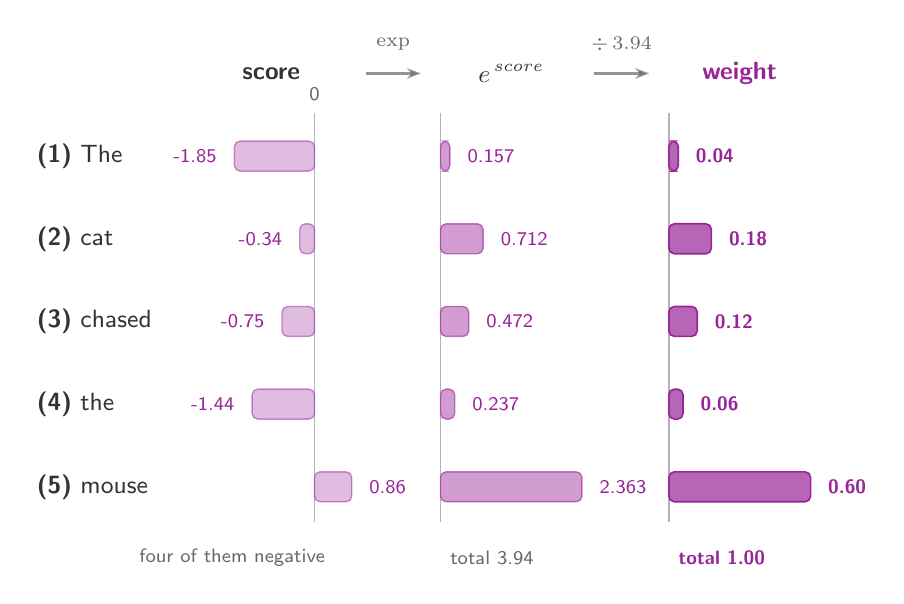
\begin{tikzpicture}[
    every node/.style={font=\sffamily},
]

% ---------------------------------------------------------------- colours
\definecolor{c1}{HTML}{15173D}
\definecolor{c2}{HTML}{982598}   % scores and weights
\definecolor{c3}{HTML}{E491C9}
\definecolor{c4}{HTML}{F1E9E9}
\definecolor{axiscolor}{HTML}{333333}
\definecolor{labelcolor}{HTML}{6B6472}

% ================================================================
%   column A  raw scores, diverging about x = 2.9   (scale 0.55)
%   column B  after exp, from x = 4.5               (scale 0.76)
%   column C  after dividing by the total, from 7.4 (scale 3.0)
%   rows      y = 5.0, 3.95, 2.9, 1.85, 0.8
% ================================================================
\def\za{2.9}   \def\sa{0.55}
\def\zb{4.5}   \def\sb{0.76}
\def\zc{7.4}   \def\sc{3.0}

% ---------------------------------------------------------------- headers
\node[font=\sffamily\small\bfseries, text=axiscolor] at (2.35, 6.05) {score};
\node[font=\sffamily\small\bfseries, text=axiscolor] at (5.4, 6.05) {$e^{\,\text{score}}$};
\node[font=\sffamily\small\bfseries, text=c2] at (8.3, 6.05) {weight};

\draw[-{Stealth[length=5pt]}, line width=1.0pt, labelcolor, opacity=0.7]
    (3.55, 6.05) -- (4.25, 6.05);
\draw[-{Stealth[length=5pt]}, line width=1.0pt, labelcolor, opacity=0.7]
    (6.45, 6.05) -- (7.15, 6.05);
\node[font=\sffamily\scriptsize, text=labelcolor] at (3.9, 6.42) {$\exp$};
\node[font=\sffamily\scriptsize, text=labelcolor] at (6.8, 6.42) {$\div\,3.94$};

% zero line for the diverging column
\draw[labelcolor, opacity=0.5, line width=0.7pt] (\za, 0.35) -- (\za, 5.55);
\node[font=\sffamily\scriptsize, text=labelcolor, anchor=south] at (\za, 5.58) {0};

% baselines for the two positive columns
\draw[labelcolor, opacity=0.5, line width=0.7pt] (\zb, 0.35) -- (\zb, 5.55);
\draw[labelcolor, opacity=0.5, line width=0.7pt] (\zc, 0.35) -- (\zc, 5.55);

% ---------------------------------------------------------------- rows
% word / y / score / exp / weight
\foreach \w/\y/\s/\e/\p in {%
    {\textbf{(1)} The}/5.0/-1.85/0.157/0.04,
    {\textbf{(2)} cat}/3.95/-0.34/0.712/0.18,
    {\textbf{(3)} chased}/2.9/-0.75/0.472/0.12,
    {\textbf{(4)} the}/1.85/-1.44/0.237/0.06,
    {\textbf{(5)} mouse}/0.8/0.86/2.363/0.60%
} {
    \node[font=\sffamily\small, text=axiscolor, anchor=west] at (-0.75, \y) {\w};

    \fill[c2, opacity=0.30, rounded corners=2pt]
        (\za, \y-0.19) rectangle (\za + \s*\sa, \y+0.19);
    \draw[c2, opacity=0.5, line width=0.5pt, rounded corners=2pt]
        (\za, \y-0.19) rectangle (\za + \s*\sa, \y+0.19);

    \fill[c2, opacity=0.45, rounded corners=2pt]
        (\zb, \y-0.19) rectangle (\zb + \e*\sb, \y+0.19);
    \draw[c2, opacity=0.6, line width=0.5pt, rounded corners=2pt]
        (\zb, \y-0.19) rectangle (\zb + \e*\sb, \y+0.19);
    \node[font=\sffamily\scriptsize, text=c2, anchor=west]
        at (\zb + \e*\sb + 0.1, \y) {\e};

    \fill[c2, opacity=0.7, rounded corners=2pt]
        (\zc, \y-0.19) rectangle (\zc + \p*\sc, \y+0.19);
    \draw[c2, line width=0.6pt, rounded corners=2pt]
        (\zc, \y-0.19) rectangle (\zc + \p*\sc, \y+0.19);
    \node[font=\sffamily\scriptsize\bfseries, text=c2, anchor=west]
        at (\zc + \p*\sc + 0.1, \y) {\p};
}

% the raw scores, on the far side of each bar
\node[font=\sffamily\scriptsize, text=c2, anchor=east] at (\za - 1.85*\sa - 0.1, 5.0) {-1.85};
\node[font=\sffamily\scriptsize, text=c2, anchor=east] at (\za - 0.34*\sa - 0.1, 3.95) {-0.34};
\node[font=\sffamily\scriptsize, text=c2, anchor=east] at (\za - 0.75*\sa - 0.1, 2.9) {-0.75};
\node[font=\sffamily\scriptsize, text=c2, anchor=east] at (\za - 1.44*\sa - 0.1, 1.85) {-1.44};
\node[font=\sffamily\scriptsize, text=c2, anchor=west] at (\za + 0.86*\sa + 0.1, 0.8) {0.86};

% ---------------------------------------------------------------- totals
\node[font=\sffamily\scriptsize, text=labelcolor, anchor=west] at (\zb, -0.1)
    {total 3.94};
\node[font=\sffamily\scriptsize\bfseries, text=c2, anchor=west] at (\zc, -0.1)
    {total 1.00};
\node[font=\sffamily\scriptsize, text=labelcolor, anchor=west] at (0.55, -0.1)
    {four of them negative};

\end{tikzpicture}
\end{document}
